\documentclass[a4paper,pagenum,english,submission]{rnti}
\usepackage{graphicx}
\usepackage{listings}

\usepackage[T1]{fontenc}
\usepackage[latin1]{inputenc}
\usepackage{url}
\usepackage{xspace}

\usepackage{xcolor}

\colorlet{punct}{red!60!black}
\definecolor{background}{HTML}{EEEEEE}
\definecolor{delim}{RGB}{20,105,176}
\colorlet{numb}{magenta!60!black}

\usepackage{tikz}
\newcommand*\circled[1]{\tikz[baseline=(char.base)]{
            \node[shape=circle,draw,inner sep=2pt] (char) {#1};}}
\newcommand{\mapapp}{\textsf{G�oCarteApp}\xspace}
\newcommand{\class}[1]{\texttt{#1}}

\lstdefinelanguage{json}{
    basicstyle=\normalfont\ttfamily,
    numbers=left,
    numberstyle=\scriptsize,
    stepnumber=1,
    numbersep=8pt,
    showstringspaces=false,
    breaklines=true,
    frame=lines,
    backgroundcolor=\color{background},
    literate=
     *{0}{{{\color{numb}0}}}{1}
      {1}{{{\color{numb}1}}}{1}
      {2}{{{\color{numb}2}}}{1}
      {3}{{{\color{numb}3}}}{1}
      {4}{{{\color{numb}4}}}{1}
      {5}{{{\color{numb}5}}}{1}
      {6}{{{\color{numb}6}}}{1}
      {7}{{{\color{numb}7}}}{1}
      {8}{{{\color{numb}8}}}{1}
      {9}{{{\color{numb}9}}}{1}
      {:}{{{\color{punct}{:}}}}{1}
      {,}{{{\color{punct}{,}}}}{1}
      {\{}{{{\color{delim}{\{}}}}{1}
      {\}}{{{\color{delim}{\}}}}}{1}
      {[}{{{\color{delim}{[}}}}{1}
      {]}{{{\color{delim}{]}}}}{1},
}


\titrecourt{\mapapp: A generic and personalized tool for the visualization of geospatial data}

\nomcourt{N. Bakerally et al.}


\titre{\mapapp: A generic and personalized tool for the visualization of geospatial data}

\auteur{Noorani Bakerally\affil{1},
        Antoine Zimmermann\affil{1},\\
				Ghislain Atemezing\affil{2}}
        

\affiliation{
    \affil{1}Univ Lyon, MINES Saint-\'Etienne, CNRS, Laboratoire Hubert Curien UMR 5516, \\F-42023 Saint-\'Etienne, France\\
          \{prenom.nom\}@emse.fr\\
    %
    \affil{2}Mondeca, \\ 35 boulevard Strasbourg, Paris, France\\
          ghislain.atemezing@mondeca.com\\
          %\http{http://www.mondeca.com}
 }

\resume{GeoSpatial data is becoming more and more important in numerous domains. A common usage of geospatial data is to visualize it on a map. For a map application to directly consume geosptial data, the data has to follow some standards or best practices such as GeoSPARQL or WSG84 vocabulary. However, there are still many datasets provided by organizations or open data portals which partly conform or do not conform at all to these standards and best practices. As a result, map application cannot directly consume them for visualization. Within many organisations, domain experts may need to visualize geospatial data from numerous heterogenous sources on a single map for analysis. As such, there is a need for a tool which consume different types of geospatial data, whether standardized, partially standard or heterogeneous to produce a map visualization. In this paper, we provide the description of such a tool, \mapapp, which can generate a default visualization of geospatial data irrespective of the model or format of the data. Moreover, we explain how further configurations can be fed input to produce personalized visualisation. Finally, we describe its usefulness in relation to the tree's dataset provided for the EGC~2017 challenge.}

%\summary{}

\begin{document}
\section{Introduction}
Currently, much data is available from open data portals and organizations. These data are encoded in different formats and based on different data models. Much of these data are geospatial data about different themes such as transportation, public services and others. Many standards and best practices such as GeoSPARQL~\citep{battle2011geosparql} or WSG84 vocabulary\footnote{\url{https://www.w3.org/2003/01/geo/wgs84_pos}} have been defined to facilitate geospatial data integration. By following these standards and best practices, geospatial applications such as map application can directly consume the data. As of now, map applications and APIs can directly consume data in standard format such GeoJSON, KML, ShapeFile and some others. For example, using Google Maps, one may drag and drop a GeoJSON data the map and directly visualize it. However, there are still many datasets provided by organizations and open data portals which partly conform or do not conform at all to these geospatial standards and best practices. As of now, datasets from open data portals are still mostly in heterogeneous format such as CSV, JSON and others. For example, simplemaps\footnote{\url{http://simplemaps.com}} provide a free dataset\footnote{\url{http://simplemaps.com/resources/world-cities-data}} about world cities together with their geospatial information in CSV. Such a dataset cannot be directly consumed for visualization purposes. Moreover, LinkedGeoData~\citep{stadler2012linkedgeodata} is a rich source of geospatial data which provides information collected by OpenStreetMap project and makes it available as RDF via their SPARQL endpoint \footnote{\url{http://linkedgeodata.org/sparql}} and RDF datasets. SPARQL queries can be written to obtain useful information from this source but the SPARQL results cannot be directly consumed by map APIs for visualization. Same is the case for GeoNames\footnote{\url{http://www.geonames.org/}} or DBpedia\footnote{\url{http://wiki.dbpedia.org/}} and other rich sources of geospatial data. To allow the map APIs to consume data from heterogeneous sources, developers have to programmatically parse the data and make it conform to the structure required by the map application or API. This task is time consuming and also requires skills and competency which may not be available by parties, such as domain experts, interested in visualizing geospatial data.

In addition, even though map APIs like Google Map have the GeoJSON Drag and Drop\footnote{\url{https://developers.google.com/maps/documentation/javascript/examples/layer-data-dragndrop}} to directly consume GeoJSON, it does not create unique colors for each layers from different sources. As a result, all marker and vector layers have the same color respectively which makes it difficult to analyse the visualization. Moreover, in GeoJSON, a features can have a number of properties. The default drag and drop feature does not consider these properties in the visualization. These properties could have been used in popups to provide some information when clicking on the layers. To customize the colors and popups for description, the API has to be programmatically exploited.

To complement all these issues, we propose a tool, \mapapp. The tool can consume geospatial data from RDF, SPARQL results and GeoJSON and produce default visualization. In the default visualization, the tool exploits data about the geospatial object to generate default description and filters which can be used for search purposes. Moreover, the tool provide a means to customize the visualization through configuration files to produce highly personalized visualizations seamlessly. In the rest of this paper, (1) we provide a description of the generic approach used by \mapapp to generate a default visualization of geospatial data in Section \ref{section:generic}; (2) we explain how this default visualization can be customized through configuration files to allow users to personalize the visualization according to their own preferences in Section \ref{section:customisation}; (3) we consider the use of \mapapp in the case of the dataset of the EGC~2017 challenge in Section \ref{section:application_grenoble}

\section{Visualizing Geospatial Data with \mapapp}\label{section:generic}
\begin{figure}
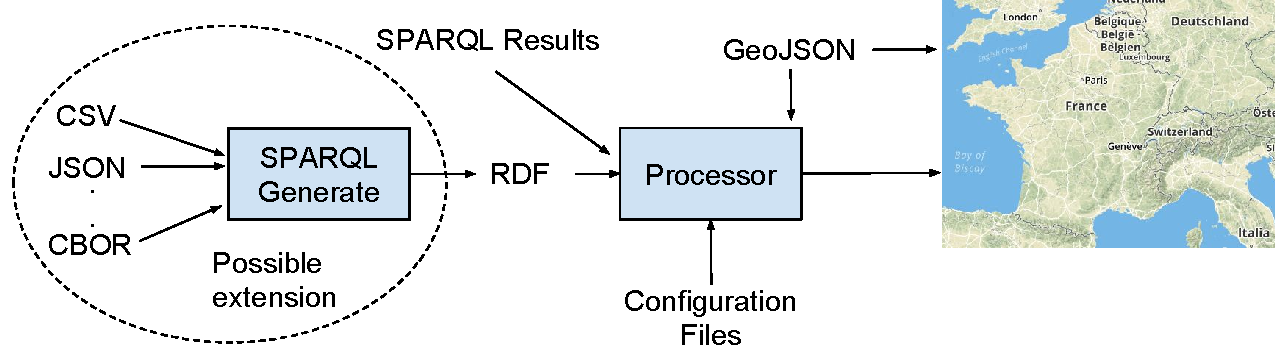
\includegraphics[scale=0.6]{img/generic_approach.pdf}
\caption{High-level view of \mapapp}
\label{fig:generic}
\end{figure}
Figure \ref{fig:generic} shows a high-level view of \mapapp. As it can be seen, \mapapp can consume data from three main sources namely RDF, SPARQL results and GeoJSON and produce a default visualization together with default filters for search purposes. As of now, the processor cannot consume data in other heterogeneous formats. But it can be further enhanced by using SPARQL Generate~\citep{Lefrancois_Zimmermann_Bakerally:16} which can produces RDF equivalent of data in formats like CSV, JSON and others. The, the RDF equivalents can then be directly input to the processor.




At the core of our tool is the processor which can process data from the three main sources and which can optionally take configuration files to produce personalized visualizations. In this section, we first provide a description of some of the classes used by the processor. Then, we explain the generic approach used by the processor to generate the default visualization. Finally, we explain how the processor can consume configuration files to produce personalized visualizations. 



\subsection{Description of the Generic Approach}
\begin{figure}
\center
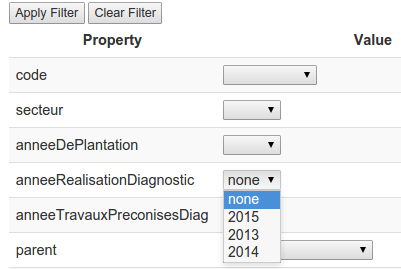
\includegraphics[scale=0.5]{img/default_filter.png}
\caption{Default filters for trees}
\label{fig:default_filter}
\end{figure}

\begin{figure}
\center
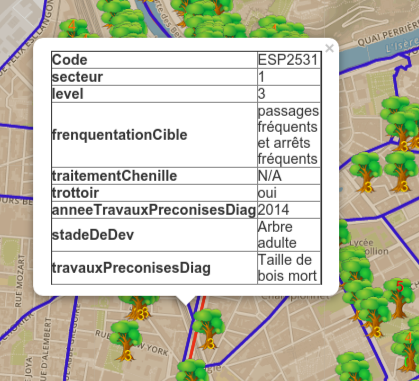
\includegraphics[scale=0.5]{img/default_description.png}
\caption{Default description for a sector in Grenoble}
\label{fig:default_description}
\end{figure}
The processor can consume geospatial data from three types of data sources and generate a default visualisation for each data source. A minimal configuration file is needed by the processor to generate a default visualization from one ore more data sources. Such a configuration will only describe the data sources, for an RDF data source and GeoJSON data source, it  specifies the URL of the RDF and GeoJSON file. For SPARQL result data source, the SPARQL endpoint URL, the query, and the variable corresponding to the latitude and longitude are specified. As sample of such a minimal configuration is shown in \ref{listing:default_configuration}. As of now, when the data source is RDF and SPARQL result, only marker items can be created, i.e. item whose type of geometry is point. When the data source is GeoJSON, all types of geometries can be considered. 

The default visualization of RDF data is possible by using WGS84 vocabulary. This means that using the default configuration, only RDF dataset using the WGS84 vocabulary can be visualized. All subjects having the predicate geo:lat and geo:long is extracted where geo is a prefix related to an IRI\footnote{\url{http://www.w3.org/2003/01/geo/wgs84_pos#}}. For each of these subject, all its other predicates are also considered. For each subject, a marker item is created. The marker item has a minimum of two properties, the latitude and the longitude. Then for each subject, the marker item also takes all its properties and and properties' values.
 
When the data source is SPARQL result, the processor queries the SPARQL endpoint with the query. For each solution in the SPARQL result, a marker item is created. As shown in Listing \ref{listing:default_configuration}, for a SPARQL result data source, the variable used as the latitude and longitude must be specified. For a particular solution, the marker item takes all the variable as its properties and corresponding variable binding as its property value. 

%For a GeoJSONDataSource, a Leaflet function is used to process the GeoJSON file. This function has callback which returns one feature and its corresponding created Layer. If the feature's geomety is a point, a MarkerDataItem is created else a VectorDataItem is created. In either case, the DataItem takes all the properties and corresponding property values for the feature. 

In a GeoJSON file, there are features which can have different types of geometries such as point or polygon. For a GeoJSON data source, the processor iterates on all the features. If the type of geometry for the feature is a point, a marker item is created else for all other geometries a vector item is created. Whether the created item is a marker item or vector item, the item takes all the properties and properties' value of the feature.
 
For a particular data source, a data item group is created which contains all the data items created from that data source. While creating data items for the data item group, the processor collects the data item properties and properties' value/s. Using this, the application can then provides a default filtering mechanism for each data item group as shown in Figure \ref{fig:default_filter}, where for each property, a set of property values is provided in a drop-down list. Property values can selected for the properties and the filter can be applied on the particular data item group. After applying the filters for a particular data item group, only those data items will be shown on the map which satisfy all the filters. As of now, a data item is shown only if its properties and property values satisfy all the filters, i.e. the filter expression is a logical AND of all the filters. This semantic can be further enhanced in future versions of the application where filter expression may be a logical OR or XOR of all filters.

The processor also generates a default description for each data item. The default description is simply a table having all property and property values, default description is binded to the map layer of the data item, on clicking on the layer, a popup is displayed as shown in Figure\ref{fig:default_description} 
\begin{lstlisting}[language=json,firstnumber=1, caption={Sample default configuration file}\label{listing:default_configuration}]
{"FranceGeoNames": {
	"dataSource": {
	"type": "RDFDataSource",
	"url": "http://www.geonames.org/3017382/about.rdf"
	}
},"Ecoles Elementaires": {
	"dataSource": {
	"type": "GeoJSONDataSource",
	"url": "http://sig.grenoble.fr/opendata/Decoupage/json/DECOUPAGE_%C3%89L%C3%89MENTAIRES_EPSG4326.json"
	}
},"Arbres": {
	"latCol": "lat",
	"longCol": "long",
	"dataSource": {
	"type": "SPARQLDataSource",
	"url": "http://data.mondeca.com/egc2017/sparql",
	"query": "The SPARQL Query goes here"
}
}}
\end{lstlisting}
\subsection{Customisation/Configuration (source)}\label{section:customisation}
\mapapp can provide a default visualization with default unique colors, filters and data item descriptions. But, the configurations can also be further customized to produce a personalized visualization. There are two types of configuration. They are:
\begin{enumerate}
\item Application configuration
\item Data configuration
\end{enumerate}
\subsubsection{Application Configuration}
The application configuration file is simple configuration which provides descriptions to bootstrap the map, for example, providing the latitude,longitude and zoom level for the initial view. As of now, these are the only simple configuration provided. We intend to extend these configuration to also include more complex configuration like specifying the map provider, i.e. whether to use Google Maps, Bing Maps\footnote{\url{https://www.bing.com/mapspreview}} or any other map providers. A sample configuration file can be found on Github\footnote{\url{https://github.com/noorbakerally/EGC2017ConfigurationFile/blob/master/app.conf}}.

\subsubsection{Data Configurations}
The datasource configuration overrides the default configuration. For example, when the data source is an RDF, by the default, the processor considers all subjects having a latitude and longitude description following the WGS84 vocabulary. However, it is possible that the RDF dataset uses a different vocabulary for latitude and longitude. To ensure that the processor finds the latitude and longitude description, two additional properties \texttt{latitudeProperty} and \texttt{longitudeProperty} can be added to the \texttt{datasource} to specify the property used for latitude and longitude respectively. 

Moreover, if the data source is SPARQL result, by default, the processor creates a unique data item for each solution. However, it is possible that a SPARQL result contains two different solutions which corresponds to a single subject. For example, this can arise if a single subject occurs in at least two different triples with the same predicates but different objects. If the default configuration is used, the processor will create a distinct data item for each solution. To prevent this, a further property \texttt{identifier} can be added to the \texttt{datasource} description to tell the processor which variable acts as the identifier. Finally, using the identifier, when the processor iterates on the SPARQL solutions, it creates a single data item for solutions having similar identifiers.

By default, the processor generates a default description for each DataItem. It is possible to configure it so that there is no description or a custom description. The custom description provided in the configuration will take the form of a string marked up with one or more properties. For example, suppose a data item has three properties namely ``code'', ``latitude'' and ``longitude'' with property values 234, 45 and 5 respectively. A custom description can be specified in the form ``The sector \{code\} has latitude \{latitude\} and longitude \{longitude\}''. The processor will then replace the property value for each of the three properties and generate a description like ``The sector 234 has latitude 45 and longitude 5''. Escape characters can be used where \{ or \} must be part of the raw string.

Also, it is possible to generate derived properties for data items. For example, in the case of Grenoble tree dataset, the year in which the tree were planted in known. It is possible to have a new property ``age'' and calculate the age of the tree. This new derived attribute can then be used both in data item's description and filters. Also, different icons and colors can be specified for data item's layers. Furthermore, layers can have different appearances like color, border color, inside color or icon based on the properties of their corresponding data item. For example, trees in different age intervals can have different icons.

As shown in Figure \ref{fig:default_filter}, there is a label for each property and for each value. These labels are taken raw as they are from the data source. As it can be seen both in Figure \ref{fig:default_filter} and \ref{fig:default_description}, the labels for the property and values follows some database or arbitrary conventions. Configurations can be used to allow for more user-friendly labels both for property and property values. Furthermore, by default, all values for a particular property are considered in the Filters' section of the user interface. In the configuration, it can be explicitly stated which property or property values to include or exclude. This can be particulary useful to omit null values or blank strings in drop-down list for property values.

It may happen that thousands of layers need to be created from one data source. Due to resource limitations, it may not be possible to show all the layers on the map. For example, in the tree dataset for EGC Challenge 2017, there are 10251 trees. Displaying all the trees may consume much resources. In this case, constraints can be introduced to limit the number of layers being rendered. As of now, we consider only one constraint which is \texttt{contains}. This constraints places a dependency between two different type of data item. For example, suppose there two data item group, one related to Grenoble Sectors and one related to the tree dataset. A \texttt{contains} constraint can be placed between on the tree dataset's data item group and Grenoble Sectors's data item group. Only those tree data item's layers are shown where a particular Grenoble Sector is visible. Therefore, to limit the number of trees shown, some sectors can be shown or hidden using filters and only trees in those sectors can be rendered.

\subsection{Classes used by the Processor}
\begin{figure}
\center
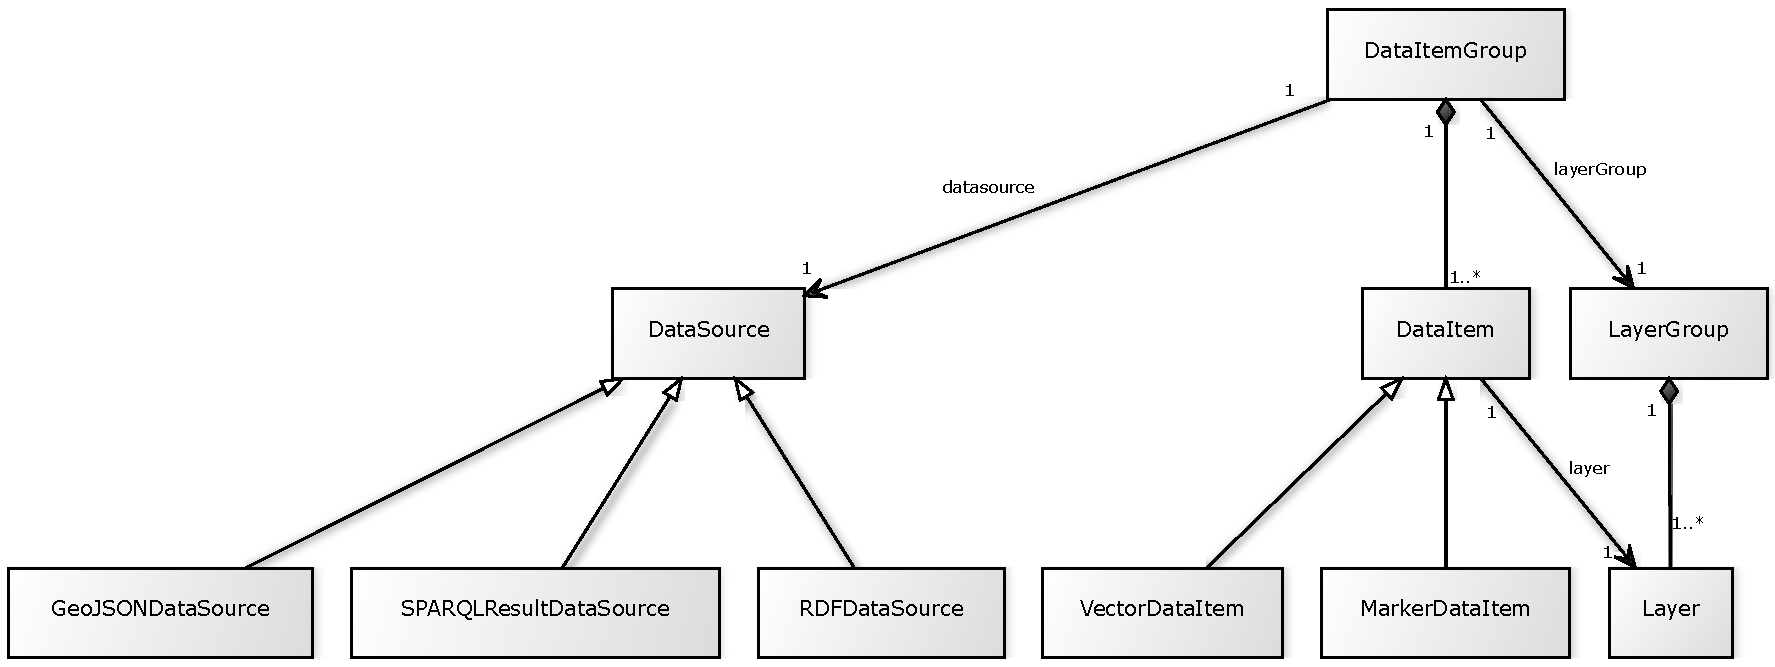
\includegraphics[scale=0.5]{img/class_diagram.pdf}
\caption{Part of \mapapp class diagram}
\label{fig:class_diagram}
\end{figure}
\mapapp is a web application written in JavaScript. It uses the JavaScript library Leaflet\footnote{\url{http://leafletjs.com/}}. The core of the application is a processor which uses the classes we defined and those defined in Leaflet. Part of the class diagram is shown in Figure \ref{fig:class_diagram}. In the class diagram, the class \class{Layer} and \class{LayerGroup} is defined within the Leaflet JavaScript Library.   

The processor can consume data from the three data sources. For each datasource, there is one \class{DataItemGroup}. For example, in Figure~\ref{fig:sample_visu}, every item in the top-right table (Area~\circled{1}) like ``Secteurs'' is an instance of \class{DataItemGroup}. A \class{DataItemGroup} contains one or more \class{DataItem}s. A \class{DataItem} contains information about one item which is shown on the map. What is shown on the map is the \class{Layer} of the \class{DataItem}. Leaflet provides the \class{LayerGroup} class which can contains one or more \class{Layer}s. On adding a \class{LayerGroup} to a map, all the Layers within it are also added. The \class{DataItemGroup} has a \class{LayerGroup} which contains all the \class{Layer} of its corresponding \class{DataItem}s. When a \class{DataItemGroup} need to shown on the map, its \class{LayerGroup}, which contains all \class{Layer}s of its \class{DataItem}s, is added to the map. As a result, all the \class{DataItem} \class{Layer}s are also added to the map.
\subsection{\mapapp: An Instantiation of the Generic Approach}
\mapapp is generic in the sense that different configuration files can be written to generate visualization for completely different datasources and personalized configurations. To show the genericity of the tool, we run the same application with two different configuration files at two different locations namely location1\footnote{\url{http://\mapapp.kissr.com/grenoble/}} and location2\footnote{\url{http://\mapapp.kissr.com/defi/}}. The two instances shows completely two different visualization. The two configuration file can be found at location1\footnote{\url{http://\mapapp.kissr.com/conf/data1.conf}} and location2\footnote{\url{http://\mapapp.kissr.com/conf/data2.conf}}. 

Figure \ref{fig:sample_visu} shows part of \mapapp. The user interface can be divided into three areas. Area~\circled{1} shows all the DataItemGroups; Area~\circled{2} shows the filters for a particular DataItemGroup and Area~\circled{3} shows the map which contains all the LayerGroups for the DataItemGroups on the map.

In the table of Area~\circled{1}, for each \class{DataItemGroup}, there is the icon to represent it on the map. It also shows the number of DataItems in that \class{DataItemGroup}. The \class{LayerGroup} for a \class{DataItemGroup} can be shown or hidden by toggling the checkbox. Finally, by pressing the button with the eye icon, the filters for that \class{DataItemGroup} is shown in Area~\circled{2}. In Area~\circled{2}, the properties for the \class{DataItem}s in the \class{DataItemGroup} are shown. The property values are available in the drop-down list. Property values for properties can be chosen and the filter can be applied to show view \class{DataItem}s having these property and property values.
 
\begin{figure}
\center
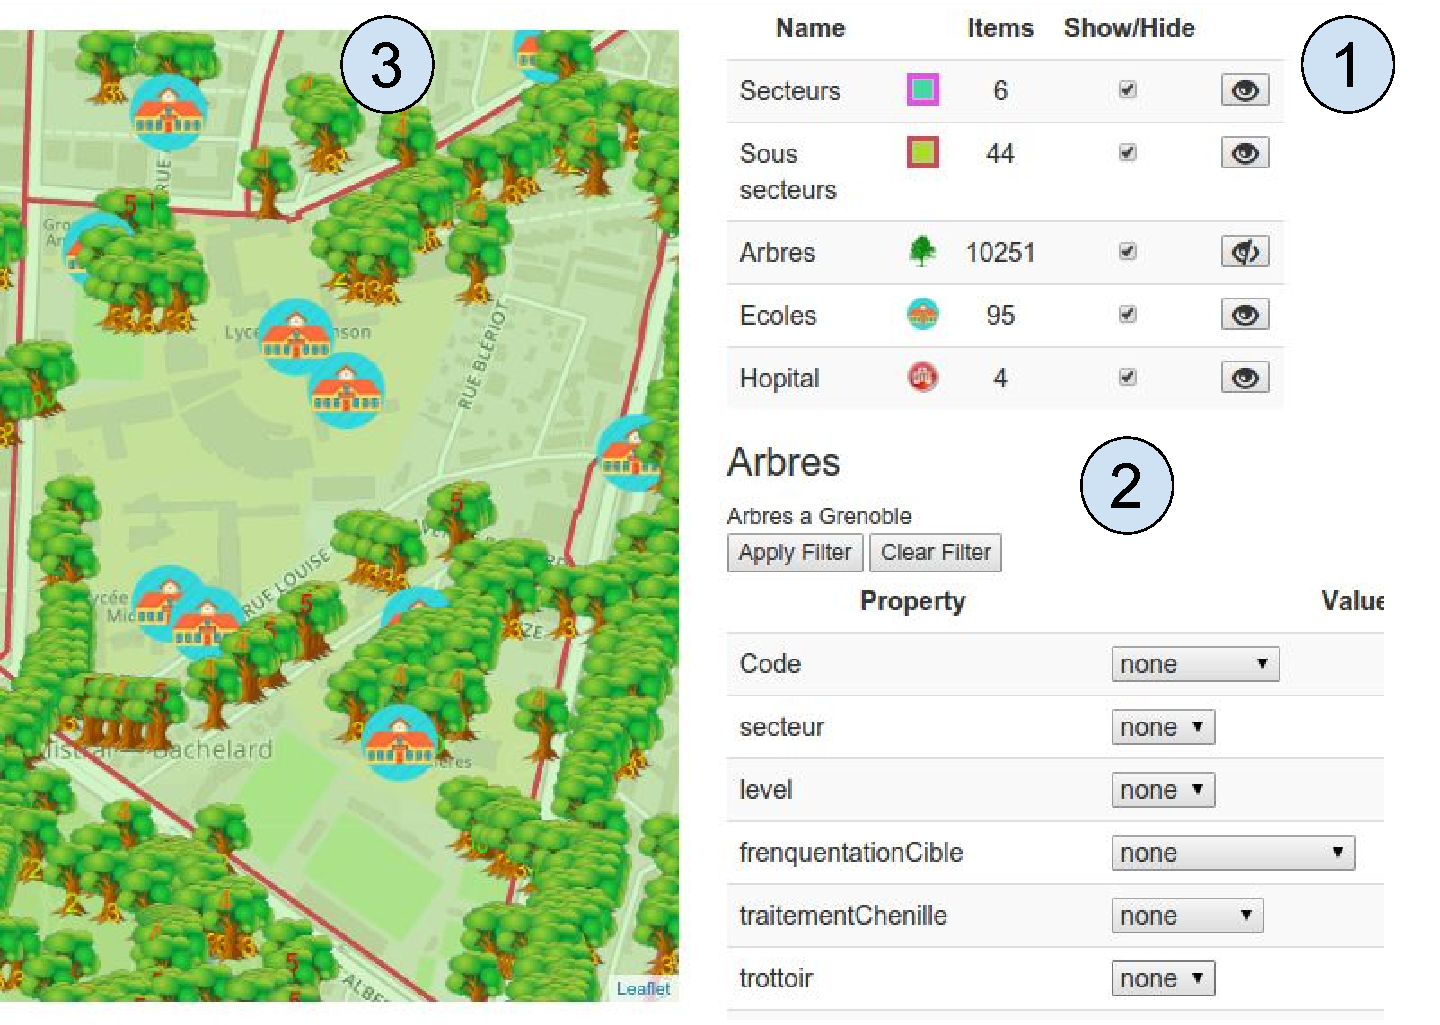
\includegraphics[scale=0.5]{img/sample_visu.pdf}
\caption{Sample screenshot of \mapapp}
\label{fig:sample_visu}
\end{figure}

\section{Application to Grenoble Data}\label{section:application_grenoble}
We apply our generic approach to visualize geospatial data in the domain of environment, in particular to monitor trees in the city of Grenoble. To that purpose, we first convert the legacy datasets into the RDF model, based on a vocabulary. Then we enrich the dataset with relevant datasets according to our use cases, and then we show how our application can be used by domain experts. Finally, we provide some recommendations on the data.

%\subsection{Transformation and Enrichment of Data}
%In this section, we explain the transformation and enrichment of the dataset provided for Defi 2. 

\subsection{Transformation}
The original datasets for Defi 2 consisted of 3 datasets. They are:
\begin{itemize}
\item File1: X\textunderscore tree\textunderscore egc\textunderscore t2.csv
\item File2: X\textunderscore geoloc\textunderscore egc\textunderscore t2.csv
\item File3: Y\textunderscore tree\textunderscore egc\textunderscore t2.csv
\end{itemize}
File1 contains details and descriptions about all the trees, File2 contains the geospatial coordinate of each trees using in EPSG{:}3945 (RGF 93/CC45). File3 contains whether the tree has any defect and if yes, where the defect is located on the tree. First of all, to transform the data, we had to change the spatial reference system from EPSG{:}3945 to EPSG{:}4326 as we chose to use the geospatial WGS84 vocabulary.

To merge all the data together in a single dataset, we had to join the each tree based on the row number in the files. This is because only File2 has a column CODE. Other files do not have this column. This step was intuitive as all the three files have the same number of rows.

Then, we provided an a model. The model use for the conversion of the CSV data is based on 2 classes, 4 object properties and 25 datatypes\footnote{\url{https://goo.gl/FTFGbh}}. We use the lgdo:Tree\footnote{\url{http://linkedgeodata.org/ontology/}} to represent the main class. The class \textit{tonto:Sector} is a sublass of a topological entity \textit{topo:EntiteTopographique}\footnote{\url{http://data.ign.fr/def/topo#}}. 

\subsection{Enrichment}
By transforming the data to RDF we can link it to external data sources with authoritative IRIs. We explain how we mapped the columns of the original CSV files to properties that link to external datasets in Table~\ref{tab:mapping}.
                                                                
\begin{table}[h!]
\caption{List of column names that provide links to external sources.}\label{tab:mapping}
\begin{tabular}{|l|l|p{6cm}|}
\hline
Column name    & Property IRI            & Note \\
\hline
ADR\_SECTEUR   & \texttt{gn{:}locatedIn} & The values are the IRIs of the \emph{cantons} from IGN.\\
CODE\_PARENT   & \texttt{gn{:}locatedIn} & We use the code to generate a new IRI to which we attach the CODE\_PARENT\_DESC by way of the property \texttt{rdfs{:}comment}.\\
ESPECE         & \texttt{dbo{:}species}  & By using DBpedia spotlight, we can map the values to the IRIs of species in DBpedia.\\
GENRE\_BOTA    & \texttt{dbo{:}genus}    & By using DBpedia spotlight, we can map the values to the IRIs of genus in DBpedia.\\
REMARQUES      & \texttt{rdfs{:}comment} & We exclude the values ``N/A'' and ``0''.\\
SOUS\_CATEGORIE& \texttt{rdf{:}type}     & We generate 4 class IRIs to which we attach the SOUS\_CATEGORIE\_DESC by way of the property \texttt{rdfs{:}comment}.\\
\hline
\end{tabular}
\end{table}

We also added information about allergy-inducing trees by mapping the botanical genus to the level of allergenic potential as found in the Wikipedia page \url{https://fr.wikipedia.org/wiki/Liste_des_plantes_allergisantes}.

In most cases, the value ``N/A'' means that the information is unknown or irrelevant, so it can be ignore. This value therefore does not generate triples. However, for some columns, ``N/A'' have a special meaning. For instance, in column TRAVAUXPRECONISESDIAG, ``N/A'' means that nothing is planned for the tree, not that the plan is unknown. In this case, we keep the ``N/A'' as an actual value for the property.
 
\subsection{Use Cases}
In this section, we provide some use cases and shows how \mapapp can be of help to domain experts in the case of Grenoble.

\subsubsection{Use Case 1}
Trees have to be maintained. In the dataset, each tree has a TRAVAUXPRECONISESDIAG, which says whether the branches have to be cut or a particular maintenance which have to be performed on the tree. Using the filters, domain experts can view trees which have to be diagnosed in a particular year. Now, they may have to decide when exactly they can go to perform the maintenance on the tree. This decision can be dependent on several parameters. For example, they may want to know whether the tree is near a school so that the maintenance can be done outside school hours. Using the DataItemGroup ``Ecole'' and ``Arbres'', all trees which have to be diagnosed in a particular year and all trees which are near to a school can be seen. 

\subsubsection{Use Case 2}
There are trees whose allergy-inducing level is known. This allergy-inducing level is scaled from 0 to 5 (from low to high allergy-inducing level). Using the filters, it is possible to find all trees with a particular allergy-inducing level whose surrounding are highly frequented by people. Moreover, it may be important to find all trees having an allergy-inducing level level of 4 or 5 and which are near to a school or hospital.

%\subsection{Recommendation on the Data}
% in French, to be translated
%Les donn�es de localisation propos�es dans ce d�fi souffrent du manque des m�tadonn�es n�cessaires pour faciliter leur exploitation, au moins sur deux aspects importants: le type de coordonn�es g�ographiques et la correspondance des (X,Y) par rapport aux latitudes et longitudes. Ces �l�ments sont fondamentaux pour faciliter la r�utilisation des donn�es g�ographiques, surtout en qui concerne le positionnement et la meilleure interpr�tation des objets contenus dans les donn�es. Il a fallu d�terminer par des scripts ad hoc que les donn�es g�ographiques utilisaient du EPSG:3945 (RGF 93/CC45) en limitant aux syst�mes de coordonn�es utilis�es en France. 
%De m�me, entre les diff�rents fichiers il n?existe pas de relation ?explicite? permettant de les relier entre elles, comme les cl�s dans les bases de donn�es. Ce manque d?information n�cessite un travail suppl�mentaire pour l?utilisateur des donn�es de faire une inf�rence bas�e sur le m�me nombre de lignes dans les diff�rents fichiers pour faire une corr�lation de similarit� bas�e sur les lignes.
%Nous pr�conisons de mettre explicitation sur les m�tadonn�es des informations de syst�mes de coordonn�es, ainsi que la mention de relations existantes entre les diff�rents fichiers � exploiter par les utilisateurs. 
%- dataset to be structured as per an ontology decided by domain experts
%- we tried to propose an ontology, however, since we lack expertise, the ontology may be erroneous
%- provide a transformation for the data from the CSV to a dataset
%- mix file together, or put identifier in the separate files
%- 


\section{Conclusion and Perspectives}
More and more geospatial data is now available with the idea of open data. This can create interesting usage use cases for both normal citizens and organizations. Map mashups can be created and provided on the Web for day to day scenarios or for analysis by domain experts. However, there is a lack of tool for the on-the-fly consumption of geospatial data in any format for visualization purposes. To our knowledge, there is no proposed approach for directly consuming geospatial data for map visualization from any data format. To this end, we propose a generic approach which can work without any configurations. We also propose the ability to define customisations in a configuration file to produce highly personalized visualization and filtering. As a proof of concept, we provide a toy application on the Web which is though not optimized but is fully function. As of now, using the application may be complex for non-technical users. This is because configuration files needs to be hand written. As a perspective, we consider the possibility of having user interfaces to help non-technical users in automatically generating configurations. Moreover, the configurations is not yet fully finalized and it will be an opportunity to have a vocabulary for to concertize the configurations and enhance its usage by interested parties. Last but not least, our future work includes the extension of this approach to consider other data formats such CSV, JSON and others. 

%\paragraph{Acknowledgements} This work has been done within the OpenSensingCity project, supported by ANR (Agence Nationale de la Recherche), Project ID: ANR-14-CE24-0029.

\bibliographystyle{rnti}
\bibliography{biblioaz}
\end{document}
